\documentclass[
    bindingoffset=5mm,  % Binding offset
    footnoteindent=3mm, % Footnote indent
    hyphenation=true    % Hyphenation turn on/off
]{tpl/wut-thesis}

\graphicspath{{src/img/}} % Images directory
\addbibresource{bibliography.bib}

\facultyeiti
\EngineerThesis
\langeng

\begin{document}

%------------------
% Title page
%------------------
\institute{TODO: Institute}
\fieldofstudy{TODO: Telecommunications?}
\specialization{TODO: Specialization}
\title{
  TODO: Thesis title
}
% Polish title
\poltitle{
  TODO: Tytuł pracy po polsku
}
\author{Błażej Sewera}
\studentnumber{300499}
\supervisor{mgr inż. Maciej Sosnowski}
\date{2022}
\maketitle

%-------------------------------------
% English abstract
%-------------------------------------
\cleardoublepage % Starting from an odd page
\abstract TODO: Abstract
\keywords XXX, XXX, XXX

%----------------------------------------
% Polish abstract
%----------------------------------------
\clearpage
\secondabstract TODO: Streszczenie po polsku
\secondkeywords XXX, XXX, XXX

\pagestyle{plain}

%--------------
% Table of Contents
%--------------
\cleardoublepage
\tableofcontents

%------------
% Sections
%------------
\cleardoublepage
\pagestyle{headings}

\hypertarget{project-management}{%
	\section{Project management}\label{project-management}}

One of the biggest challenges turned out to be non-technical. Project
management even with only one person can be difficult, as it requires a
great amount of self-discipline. Luckily, there were some tools and
processes that helped with this task.

\hypertarget{product-development}{%
	\subsection{Product development}\label{product-development}}

The most important thing I learned from project management was
undoubtedly how to reliably conduct product development. When I started
developing Notipie, I had a very vague vision of what the finish product
will provide. The essential functionality was interleaved with features
that could not be implemented without the essentials.

That is when I decided to streamline the development and set a
constraint of what needs to be done in order to consider the product
usable. I defined the \textbf{Minimally Viable Product} and prioritized
the issues\footnote{Issues with the MVP milestone, retrieved 2022-05-29.
	\url{https://github.com/blazejsewera/notipie/issues?q=is\%3Aissue+milestone\%3AMVP}}.

\hypertarget{minimally-viable-product}{%
	\subsubsection{Minimally Viable
		Product}\label{minimally-viable-product}}

The definition is as follows\footnote{MVP milestone, retrieved
	2022-05-29. \url{https://github.com/blazejsewera/notipie/milestone/1}}:

\begin{quote}
	Notifications can be sent with a manually programmed script with the
	help of a library. They arrive to the user interface in real time.
	
	The library is provided in the MVP.\\
	The backend correctly forwards those notifications to the frontend.\\
	The backend stores existing notifications on the disk.\\
	The frontend correctly presents notifications to the user.
\end{quote}

\hypertarget{project-board}{%
	\subsection{Project board}\label{project-board}}

One of the great tools that helped with the project management was the
new Github Project board, which is currently in beta\footnote{Github
	Projects (beta) documentation, retrieved 2022-05-29.
	\url{https://docs.github.com/en/issues/trying-out-the-new-projects-experience/about-projects}}.
The Kanban board\footnote{Kanban board -- article on Wikipedia,
	retrieved 2022-05-29. \url{https://en.wikipedia.org/wiki/Kanban_board}}
consists of four sections (columns):

\begin{itemize}
	\item
	      Todo
	\item
	      Open
	\item
	      In Progress
	\item
	      Done
\end{itemize}

Section \textbf{Todo} consists of all the issues connected to this
project that are planned to be worked on in the future.

Section \textbf{Open} consists of issues that need to be worked on next.
Those are usually one to three issues that need to be done in a certain
order.

Section \textbf{In Progress} contains issues that are currently being
worked on. There is usually only one issue in this column.

Section \textbf{Done} consists of all the finished issues, as well as
the issues that were decided to be unnecessary. In that case, the issues
are marked with a \texttt{wontfix} label.

\hypertarget{backend-core}{%
	\section{Backend (core)}\label{backend-core}}

The backend's code is in the \texttt{core} directory\footnote{The
	\texttt{core} directory, retrieved 2022-05-31.
	\url{https://github.com/blazejsewera/notipie/tree/master/core}}.

\hypertarget{core-project-architecture}{%
	\subsection{Core project architecture}\label{core-project-architecture}}

The project on the top-level is structured over 4 directories:

\begin{itemize}
	\item
	      \texttt{cmd} -- entry point to the application (\texttt{main})
	\item
	      \texttt{internal} -- application-specific code
	\item
	      \texttt{pkg} -- reusable utils, not specific to the application
	\item
	      \texttt{test} -- black box integration test code
\end{itemize}

\hypertarget{the-internal-directory}{%
	\subsubsection{\texorpdfstring{The \texttt{internal}
		directory}{The internal directory}}\label{the-internal-directory}}

Application-specific code is split into 5 directories representing the
levels of abstraction:

\begin{itemize}
	\item
	      \texttt{domain} -- business logic, defines data structures and
	      communication of domain objects on the highest level of abstraction,
	\item
	      \texttt{grid} -- lower level of abstraction than domain, defines
	      proxies that convert network models into domain models, creates and
	      organizes domain objects into a grid, in which those objects can
	      communicate,
	\item
	      \texttt{impl} -- implements network endpoints, WebSockets, and
	      persistence,
	\item
	      \texttt{infra} -- configures the application and sets up the context
	      for DI,
	\item
	      \texttt{model} -- defines network data models.
\end{itemize}

\hypertarget{go-in-core}{%
	\subsection{Go in core}\label{go-in-core}}

Go is quickly gaining popularity among developers, with its great
tooling, focus on microservices, and state-of-the-art standard library.

\hypertarget{motivation}{%
	\subsubsection{Motivation}\label{motivation}}

When choosing the right language for the project, I focused on finding
the right tool for the application and developer experience.

I wanted \texttt{notipie} to be a high-performance microservice, so I
did not take interpreted languages like Python or JavaScript into
consideration. I mostly considered Java, Kotlin, Rust, and Go.

Java, although popular, does not have the greatest developer experience.
Things like \texttt{equals} and \texttt{hashCode} are unnecessary bloat
in the code. Project Lombok fixes some of them, but the tooling is
limited to IntelliJ, you have to download a lot of libraries for dealing
with JSON, create your own code style guide, and perform a fair bit of
setup.

Kotlin, far better than Java, but also locked-in to IntelliJ with
tooling, was an interesting option for me, but not ideal.

Rust was too low-level for my application. Explicit memory management,
although performant, was simply too verbose and work-intensive for my
use case.

Go was a perfect option. A plethora of great tooling, like first-party
Go plugin for VSCode, GoLand from JetBrains, community plugins for
Neovim, all working great and providing a good developer experience.
Furthermore, extraordinary performance of the tooling itself, with tests
running in under a second, super-fast compiler, one of the best standard
libraries I have seen, and overall simplicity of the language, made the
choice obvious.

\hypertarget{how-did-go-make-the-development-easier}{%
	\subsubsection{How did Go make the development
		easier}\label{how-did-go-make-the-development-easier}}

\hypertarget{built-in-language-features}{%
	\paragraph{Built-in language
		features}\label{built-in-language-features}}

The feature that helped the most during development was channels and
\emph{goroutines}, coroutines automatically managed by the Go runtime.
The idea behind those was very simple to understand, and working with
concurrent programming was a little bit easier.

\hypertarget{standard-library}{%
	\paragraph{Standard library}\label{standard-library}}

Standard \texttt{testing} package provides a unified, and simple tooling
for testing. I did not have to think anything about test setup. No
custom scripts, third-party libraries, or IDE setup. All I needed to do
was to name a file with \texttt{\_test.go} suffix, write a function
starting with \texttt{Test}, and run \texttt{go\ test\ ./...}. Both
VSCode with Go plugin, and GoLand automatically picked up the test setup
and I was ready to develop with TDD.

Standard \texttt{net/http} package provides everything needed for
setting up REST endpoints. Although I used Gin\footnote{Gin web
	framework, retrieved 2022-05-31. \url{https://gin-gonic.com}} for
this, due to a simpler interface, I used status codes and HTTP client
implementation from \texttt{net/http}.

\hypertarget{third-party-libraries}{%
	\paragraph{Third-party libraries}\label{third-party-libraries}}

Gin was great for writing REST endpoints, with \texttt{gin.Context}
having easy access to standard-library-compatible fields, making it
easily pluggable to other third-party libraries, like Gorilla
WebSocket\footnote{Gorilla WebSocket implementation, retrieved
	2022-05-31. \url{https://github.com/gorilla/websocket}}.

Zap\footnote{Zap, the logging library, retrieved 2022-05-31.
	\url{https://github.com/uber-go/zap}} provided an excellent and
performant way to log things in the backend. Structured logging,
automatic serialization to JSON in production mode, and human-readable
format in debug mode, paired with low or zero-allocation overhead, made
it a perfect choice for logging in a microservice.

\hypertarget{frontend-ui}{%
	\section{Frontend (ui)}\label{frontend-ui}}

\hypertarget{ui-design}{%
	\subsection{UI Design}\label{ui-design}}

When designing the UI of Notipie, I tried to maximize usability, and
minimize complexity of the interface.

\hypertarget{inspirations}{%
	\subsubsection{Inspirations}\label{inspirations}}

My main inspirations for the interface were Apple Human Interface
Guidelines\footnote{Apple Human Interface Guidelines, retrieved
	2022-05-31.
	\url{https://developer.apple.com/design/human-interface-guidelines/}}
and Google's Material Design\footnote{Google's Material Design,
	retrieved 2022-05-31. \url{https://material.io}}, but by far the most
inspiration was taken from Github Primer\footnote{Github Primer,
	retrieved 2022-05-31. \url{https://primer.style}}.

I tried to break down what is useful, what is unnecessary in my project,
and extract only the essentials for my design.

\hypertarget{final-design}{%
	\subsubsection{Final design}\label{final-design}}

\hypertarget{the-card}{%
	\paragraph{The card}\label{the-card}}

The card is a building block for the entire user interface. It provides
the most interaction in the whole application, therefore it had to be
designed with clearly laid out information and intuitive controls.

\begin{figure}
	\centering
	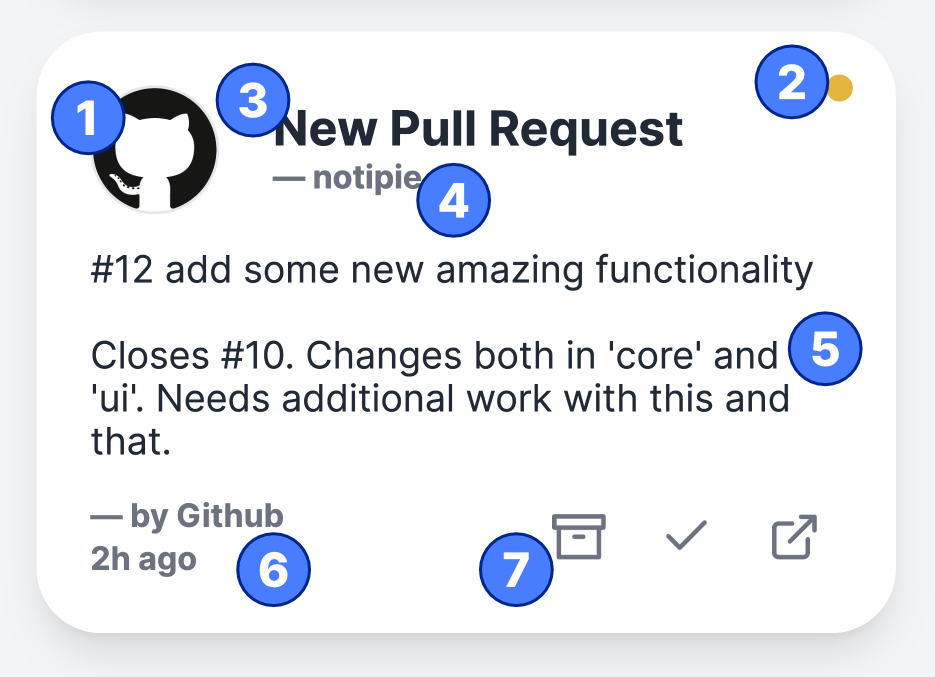
\includegraphics[width=8cm,height=\textheight]{./img/card_labeled.png}
	\caption{The card with labeled elements}
\end{figure}

The card itself consists of several elements:

\begin{enumerate}
	\item
	      logo, it can be an image or automatically generated SVG from the first
	      two letters of the app's name,
	\item
	      indicator, whether the notification has been seen or not,
	\item
	      title of the notification,
	\item
	      subtitle,
	\item
	      body, that collapses after it reaches a certain length, so that an
	      ellipsis appears (\texttt{{[}...{]}}),
	\item
	      information about what app sent the notification and when it happened,
	\item
	      controls to archive, mark as read, or go to external site connected
	      with the notification, like a certain build on Jenkins, or the
	      notification page on Github.
\end{enumerate}

\begin{figure}
	\centering
	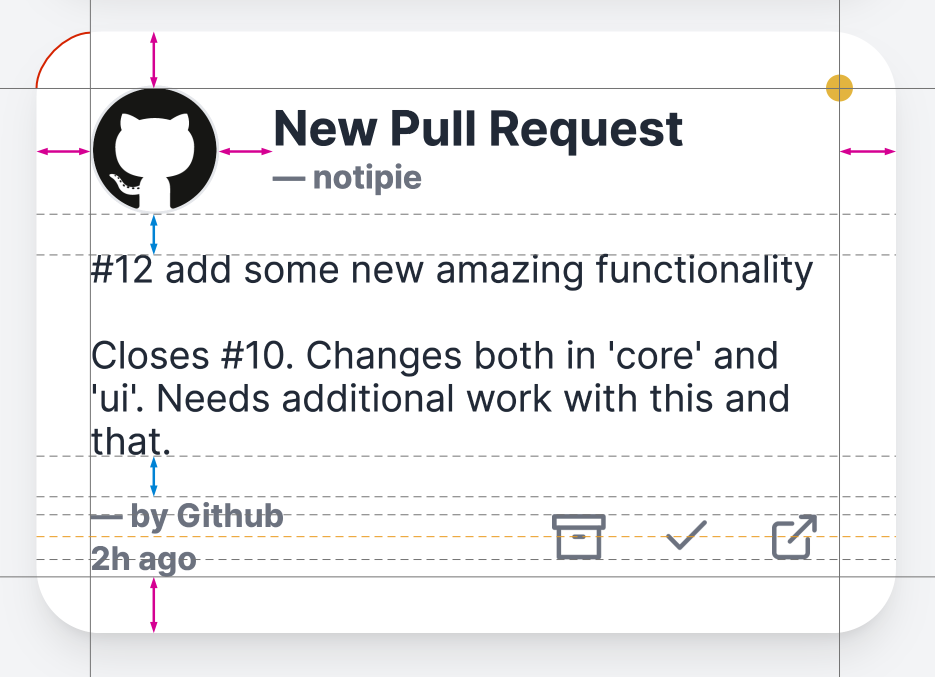
\includegraphics[width=8cm,height=\textheight]{./img/card_guides.png}
	\caption{The card with guides}
\end{figure}

The card was also designed with aesthetics in mind. All elements were
carefully positioned and aligned, so they are not only pleasant to look
at, but also have some features important for visual communication:

\begin{itemize}
	\item
	      the rounded corners take the focus away from the card frame, and
	      provide a natural, neutral enclosure for the notification,
	\item
	      the inner padding is of equal size in each direction to provide
	      optical stability,
	\item
	      the distance between the logo and title -- subtitle combo is the same
	      size as the padding, making the logo appear centered,
	\item
	      the title -- subtitle combo itself is centered vertically relative to
	      the logo,
	\item
	      the distances between the logo, notification body, and app name --
	      timestamp combo are shorter in order to make the inner section more
	      connected,
	\item
	      the controls are centered relative to the app name -- timestamp combo,
	\item
	      the \emph{unread} indicator is unobtrusive enough not to steal all the
	      focus from the card's content,
	\item
	      finally, the \emph{unread} indicator is positioned slightly outside
	      the inner section, so that it belongs to the card itself, not its
	      content, therefore it is easier to spot at a glance.
\end{itemize}

\hypertarget{ui-component-library}{%
	\subsection{UI component library}\label{ui-component-library}}

When choosing the library for the UI components, I considered:

\begin{itemize}
	\item
	      React\footnote{React, retrieved 2022-05-31. \url{https://reactjs.org/}},
	\item
	      Vue.js\footnote{Vue.js, retrieved 2022-05-31. \url{https://vuejs.org/}},
	      and
	\item
	      Angular\footnote{Angular, retrieved 2022-05-31.
	      	\url{https://angular.io/}}.
\end{itemize}

All those libraries are very popular, so I chose React, because I had
the most experience with it in my professional work.

\hypertarget{ui-networking}{%
	\subsection{UI networking}\label{ui-networking}}

The nature of notifications required me to use both REST data fetching
and asynchronous data pushes from the backend. For the latter, I decided
to use WebSockets, a standard defined in RFC6455\footnote{RFC6455,
	retrieved 2022-05-31.
	\url{https://www.rfc-editor.org/rfc/rfc6455.html}}, and
RxJS\footnote{RxJS, retrieved 2022-05-31. \url{https://rxjs.dev/}}, an
implementation of ReactiveX library\footnote{ReactiveX library,
	retrieved 2022-05-31. \url{https://reactivex.io/}}.

\hypertarget{rest-data-fetching}{%
	\subsubsection{REST data fetching}\label{rest-data-fetching}}

I used simple REST\footnote{REST definition, MDN Web Docs, retrieved
	2022-05-31.
	\url{https://developer.mozilla.org/en-US/docs/Glossary/REST}} requests
for fetching the notifications that are already on the backend server.
The standard Fetch browser API\footnote{Fetch browser API, retrieved
	2022-05-31.
	\url{https://developer.mozilla.org/en-US/docs/Web/API/Fetch_API}} was
sufficient for the task.

\hypertarget{reactive-raven}{%
	\subsubsection{Reactive Raven}\label{reactive-raven}}

This project\footnote{Reactive Raven, retrieved 2022-05-31.
	\url{https://github.com/blazejsewera/reactive-raven}} was an
experiment on using RxJS for all real-time data fetching, enabling the
separation of concerns in the code, and decoupling the state management
implementation from the networking implementation.

When searching for the optimal solution for pushing the data to the UI,
I came across two major solutions:

\begin{itemize}
	\item
	      Redux Thunks -- okay for fetching some data on user interaction,
	      e.g.~on a button click, but it provides virtually full implementation
	      lock-in, and very little separation of concerns. Fetching data is an
	      action dispatched on a store, so external communication and storing
	      data are dependent on each other.
	\item
	      Redux Sagas -- good for managing side effects with plain JavaScript,
	      but they use generator functions that yield a different type every
	      time, so they are very problematic to use with strict TypeScript.
\end{itemize}

Both thunks and sagas did not provide the separation of concerns I
wanted to achieve. Fetching or acting upon pushed data is a different
concern than storing it.

As a user, I should not have to dispatch an action on a store, when I
want to fetch data. Of course, the data can be immediately stored after
fetching, but this behavior should be injected later, so that there is
no store implementation lock-in.

This separation of concerns enabled me to migrate from Redux to Zustand
as my \emph{store} implementation, as described in the next section.

\hypertarget{state-management-in-ui}{%
	\subsection{State management in UI}\label{state-management-in-ui}}

To simplify the frontend code, I needed to use a single source of truth
for the data. I used both Redux\footnote{Redux, retrieved 2022-05-31.
	\url{https://redux.js.org/}}, and Zustand\footnote{Zustand, retrieved
	2022-05-31. \url{https://github.com/pmndrs/zustand}} for this task as
\emph{store} implementations, and Zustand came on top as a simpler
solution for my application.

\hypertarget{redux}{%
	\subsubsection{Redux}\label{redux}}

Redux is great for big applications with lots of components. Being one
of the most popular state management libraries for React, it was my
first choice.

Unfortunately, it required me to write a lot of boilerplate code, and
thus was not easily maintainable for a smaller project like Notipie.

\hypertarget{zustand}{%
	\subsubsection{Zustand}\label{zustand}}

Zustand is a lot simpler than Redux, requires a lot less boilerplate
code, and was sufficient for my application. I migrated to it in commit
\texttt{7677d13}\footnote{commit \texttt{7677d13}, retrieved 2022-05-31.
	\url{https://github.com/blazejsewera/notipie/commit/7677d1335d23994d3563d7672982b5aaf72fbbca}},
and it reduced the lines of code by over 200. I did not however give up
the connected components, as they provide better testability and
separation of concerns, which is worth a bit extra code for that.

\hypertarget{typescript-in-ui}{%
	\subsection{TypeScript in UI}\label{typescript-in-ui}}

I decided to use TypeScript in my project for the frontend part because
of its type checking tools, huge popularity, and a growing demand for in
on the job market.

\hypertarget{choosing-the-language}{%
	\subsubsection{Choosing the language}\label{choosing-the-language}}

When choosing which language to use in the UI, I considered a couple of
options:

\begin{itemize}
	\item
	      plain JavaScript,
	\item
	      TypeScript,
	\item
	      Elm, and
	\item
	      CoffeeScript.
\end{itemize}

I immediately discarded the last two, due to their smaller popularity
compared to JavaScript or TypeScript.

The featureset of the language was also very important to me. JavaScript
is by far the most popular, but it lacks type annotations or pre-runtime
type checking. TypeScript and Elm turned out to be winners in the type
checking toolchain.

TypeScript also has a big advantage of being very similar to plain
JavaScript, so the transpiled code is very readable.

A big factor was general trend of language's popularity growth.
TypeScript was a clear winner in this scenario, being third most loved
language and second most wanted language in the Stack Overflow Developer
Survey 2021\footnote{Stack Overflow Developer Survey 2021, retrieved
	2022-05-31.
	\url{https://insights.stackoverflow.com/survey/2021\#most-loved-dreaded-and-wanted-language-want}}.
It was only beaten by Rust and Clojure in the \emph{Most Loved} section,
both of which are non-frontend languages, and Python in the \emph{Most
Wanted} section, which is also not a frontend language.

Another report confirming the growing popularity of TypeScript is Github
Octoverse Report 2021\footnote{Github Octoverse Report 2021, retrieved
	2022-05-31.
	\url{https://octoverse.github.com/\#top-languages-over-the-years}}.
Since 2017 it beat Ruby, C, C++, C\#, Shell, and PHP and is, as of 2021,
fourth top language on Github.

\hypertarget{working-with-typescript}{%
	\subsubsection{Working with TypeScript}\label{working-with-typescript}}

Starting with TypeScript was fairly easy, the toolchain was included in
the project creation scripts. Most dependencies had good TypeScript
annotations, or they were completely written in TypeScript, which was
very helpful for maintaining type safety.

Learning the language was also very easy. I was already familiar with
JavaScript, so I only needed to learn the type annotations, which were
very intuitive to use.

\hypertarget{build-system}{%
	\subsection{Build system}\label{build-system}}

For the build and bundle software, I wanted to use something modern,
with hot module reloading, easy to use setup scripts, customizable
development server, and short bundle times.

\hypertarget{snowpack-and-vite}{%
	\subsubsection{Snowpack and Vite}\label{snowpack-and-vite}}

I started with Snowpack\footnote{Snowpack, retrieved 2022-05-31.
	\url{https://www.snowpack.dev}} and used it until I decided to move to
Vite\footnote{Vite, retrieved 2022-05-31. \url{https://vitejs.dev}} in
commit \texttt{c11bc35}\footnote{commit \texttt{c11bc35}, retrieved
	2022-05-31.
	\url{https://github.com/blazejsewera/notipie/commit/c11bc35370f512f35d522a55fcd216c1c80ea75a}}.

Snowpack offered both hot module reloading and short bundle times,
however, there were some minor problems from time to time, the project
had a slow development, and the alternative, Vite did not seem to have
those problems.

I tried Vite in my other project, Reactive Raven\footnote{Reactive
	Raven, retrieved 2022-05-31.
	\url{https://github.com/blazejsewera/reactive-raven}}, and the
integration with React, TypeScript, Tailwind CSS, and other tools I used
was seamless, therefore I decided to migrate to it in Notipie as well.

On April 20th, 2022, Snowpack's maintainer stated in the project's
Readme document (commit \texttt{45456aa})\footnote{project's Readme
	document (commit \texttt{45456aa}), retrieved 2022-05-31.
	\url{https://github.com/FredKSchott/snowpack/blob/45456aa14978460afcb5ce20f7296556d22c7595/README.md}}
that they would no longer maintain the project and mentioned Vite as a
good alternative for it.


 % Można też pisać rozdziały w jednym pliku.
\clearpage % Zawsze zaczynamy rozdział od nowej strony
\section{Summary}
TODO: Summary

%---------------
% Bibliography
%---------------
\cleardoublepage
\printbibliography
\clearpage

% Acronym list
% TODO: Remember to sort acronyms alphabetically manually!
\acronymlist
\acronym{EiTI}{Wydział Elektroniki i Technik Informacyjnych}
\acronym{PW}{Politechnika Warszawska}
\vspace{0.8cm}

%------------------------------------------
% Lists of figures, tables, and appendices
%------------------------------------------
\pagestyle{plain}

\listoffigurestoc
\vspace{1cm}
\listoftablestoc
\vspace{1cm}
\listofappendicestoc

%-------------
% Appendices
%-------------

%% Figures and tables in appendices are not listed
% \captionsetup[figure]{list=no}
% \captionsetup[table]{list=no}

%% Example Appendix 1
% \clearpage
% \appendix{Appendix name 1}
% \begin{figure}[!h]
% 	\centering \includegraphics[width=0.5\linewidth]{logopw2.png}
% 	\caption{Obrazek w załączniku.}
% \end{figure}

%% Example Appendix 2
% \clearpage
% \appendix{Appendix name 2}
% \begin{table}[!h] \centering
%     \caption{Tabela w załączniku.}
%     \begin{tabular} {| c | c | r |} \hline
%         Kolumna 1       & Kolumna 2 & Liczba \\ \hline\hline
%         cell1           & cell2     & 60     \\ \hline
%         \multicolumn{2}{|r|}{Suma:} & 123,45 \\ \hline
%     \end{tabular}
% \end{table}

\end{document} % Goodnight
